% ============================================================
%  CSE200 Online-1 (B1)  ->  "Laplace Analysis and Applications"
%  Assets in this folder:  rc_circuit.png   rc_response.py   laplace.bib
%  Compile:  pdflatex Q4_Laplace.tex   (twice, for cross-references)
% ============================================================
\documentclass[11pt]{article}

\usepackage[T1]{fontenc}
\usepackage[utf8]{inputenc}
\usepackage[margin=1in]{geometry}
\usepackage{amsmath}
\usepackage{amssymb}
\usepackage{mathtools}
\usepackage{graphicx}
\usepackage{wrapfig}
\usepackage{xcolor}
\usepackage{multirow}
\usepackage{array}
\usepackage{enumitem}
\usepackage{listings}      % code listings
\usepackage{hyperref}

\hypersetup{colorlinks=true, linkcolor=black, citecolor=black, urlcolor=blue}

% ---- Python listing style ---------------------------------
\lstdefinestyle{pystyle}{
    language=Python,
    basicstyle=\ttfamily\small,
    keywordstyle=\color{blue!70!black}\bfseries,
    stringstyle=\color{red!65!black},
    commentstyle=\color{green!45!black}\itshape,
    numbers=left,
    numberstyle=\tiny\color{gray},
    numbersep=8pt,
    frame=single,
    rulecolor=\color{gray!60},
    breaklines=true,
    showstringspaces=false,
    tabsize=4
}

\title{Laplace Analysis and Applications}
\author{Pierre-Simon Laplace\textsuperscript{1}, Oliver Heaviside\textsuperscript{2},
        and Gustav Robert Kirchhoff\textsuperscript{3}\\[0.6em]
        \textsuperscript{1}Acad\'emie des Sciences, Paris, France\\
        \textsuperscript{2}Royal Society, London, United Kingdom\\
        \textsuperscript{3}University of Heidelberg, Heidelberg, Germany}
\date{}

\begin{document}
\maketitle

% ------------------------------------------------------------
\section{From Functions to Transforms}

\subsection{The Laplace Transform}
Let $f(t)$ be a function defined for $t \ge 0$. Its Laplace transform is defined by
\begin{equation}\label{eq:def}
    \mathcal{L}\{f(t)\} = F(s) = \int_0^\infty e^{-st} f(t)\,\mathrm{d}t, \qquad s > 0.
\end{equation}
The transform changes a function of time into a function of the new variable
$s$.\footnote{The variable $s$ is commonly interpreted as a complex-frequency
variable.} Symbolically,
\[
    f(t) \xrightarrow{\ \ \mathcal{L}\ \ } F(s).
\]
The inverse Laplace transform reverses this process:
\begin{equation}
    f(t) = \mathcal{L}^{-1}\{F(s)\}.
\end{equation}
The main purpose of the method is to replace differentiation and integration in
the time domain by simpler algebraic operations in the transform
domain~\cite{kreyszig2011}. A concise overview is available from the
\href{https://mathworld.wolfram.com/LaplaceTransform.html}{Laplace Transform entry
on MathWorld}.

\subsection{A Simple Example}
For the constant function $f(t) = 1$,
\begin{equation}
    \begin{split}
        \mathcal{L}\{1\} &= \int_0^\infty e^{-st}\,\mathrm{d}t \\
                         &= \left[-\frac{1}{s} e^{-st}\right]_0^\infty \\
                         &= \frac{1}{s}.
    \end{split}
\end{equation}
Similarly,
\begin{equation}
    \mathcal{L}\{t\} = \frac{1}{s^2}, \qquad \mathcal{L}\{t^2\} = \frac{2}{s^3}.
\end{equation}

% ------------------------------------------------------------
\section{Common Transform Equations}
Table~\ref{tab:laplace} lists several frequently used Laplace-transform equations.

\begin{table}[ht]
    \centering
    \caption{Selected Laplace-transform equations.}
    \label{tab:laplace}
    \begin{tabular}{|c|c|c|c|}
        \hline
        \multirow{2}{*}{\textbf{Family}}
            & \multicolumn{2}{c|}{\textbf{Transform Equation}}
            & \multirow{2}{*}{\textbf{Condition}} \\
        \cline{2-3}
            & \textbf{Time function} & \textbf{Laplace transform} & \\
        \hline
        \multirow{3}{*}{Algebraic}
            & $1$   & $\dfrac{1}{s}$          & $s > 0$ \\
        \cline{2-4}
            & $t$   & $\dfrac{1}{s^2}$        & $s > 0$ \\
        \cline{2-4}
            & $t^n$ & $\dfrac{n!}{s^{n+1}}$   & $n = 0, 1, 2, \dots$ \\
        \hline
        \multirow{2}{*}{Exponential}
            & $e^{at}$  & $\dfrac{1}{s-a}$ & $s > a$ \\
        \cline{2-4}
            & $e^{-at}$ & $\dfrac{1}{s+a}$ & $s > -a$ \\
        \hline
        \multirow{2}{*}{Oscillatory}
            & $\sin(\omega t)$ & $\dfrac{\omega}{s^2+\omega^2}$ & $\omega > 0$ \\
        \cline{2-4}
            & $\cos(\omega t)$ & $\dfrac{s}{s^2+\omega^2}$      & $\omega > 0$ \\
        \hline
        \multicolumn{2}{|c|}{\textbf{Unit-step function} $u(t-a)$}
            & $\dfrac{e^{-as}}{s}$ & $a > 0$ \\
        \hline
    \end{tabular}
\end{table}

The formulas in Table~\ref{tab:laplace} allow many functions to be transformed
without repeatedly evaluating improper integrals.

% ------------------------------------------------------------
\section{Application to an RC Circuit}

\subsection*{Circuit Model}
\begin{wrapfigure}{r}{0.45\textwidth}
    \centering
    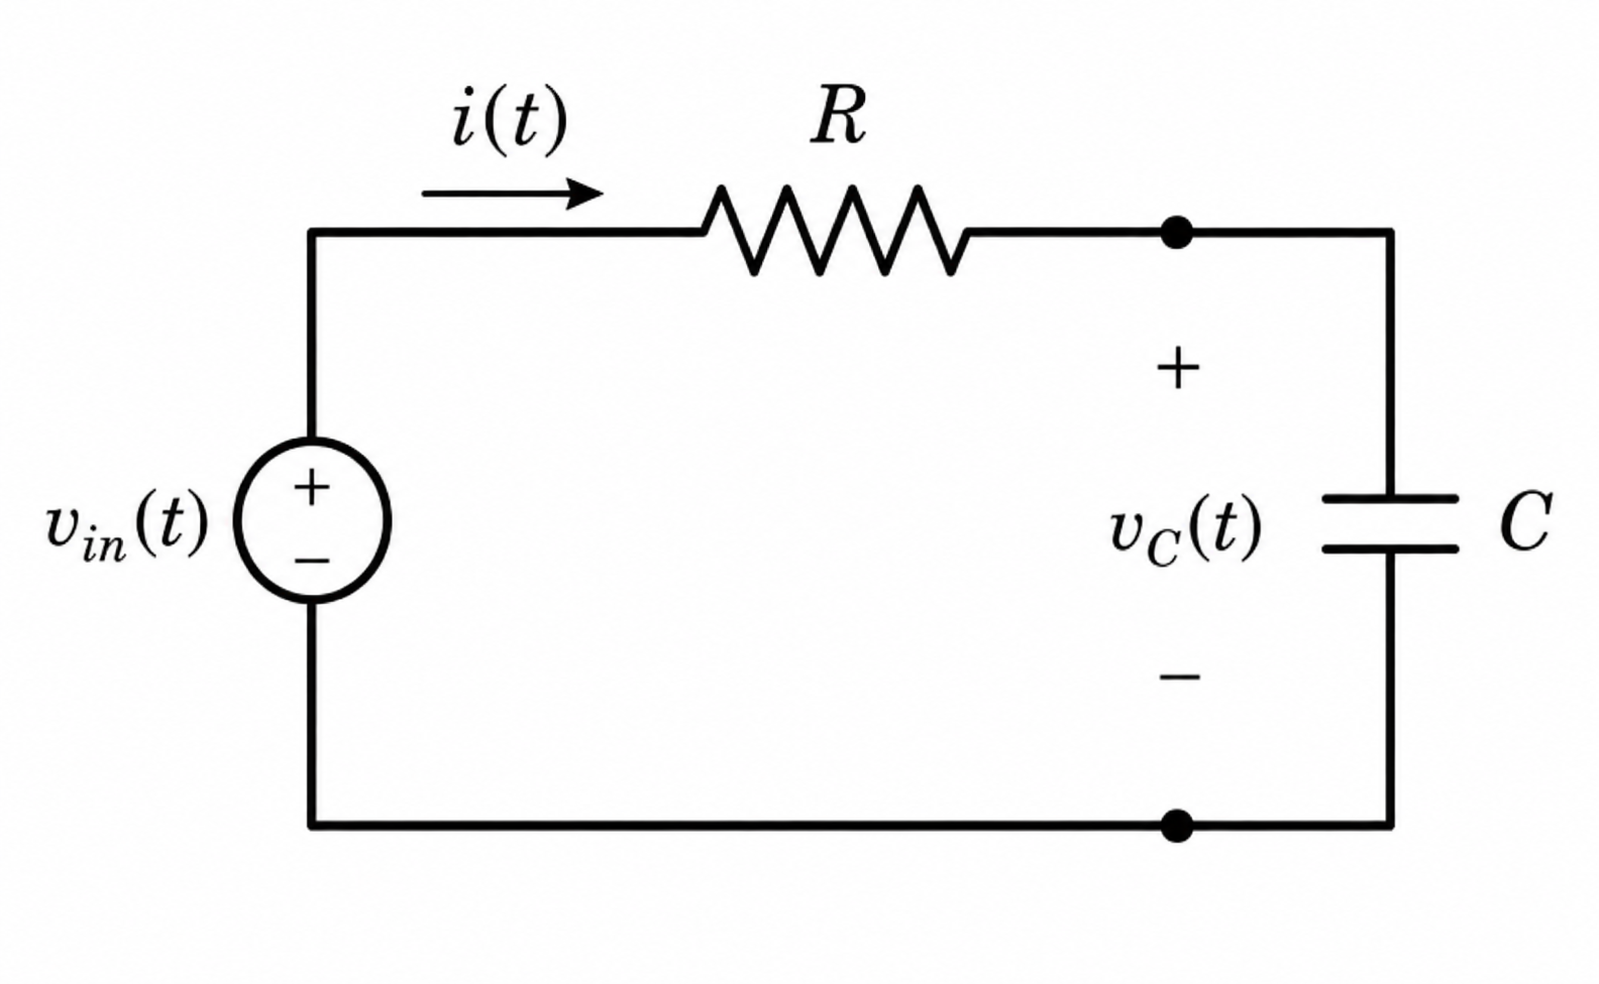
\includegraphics[width=0.43\textwidth]{rc_circuit.png}
    \caption{A simple series RC circuit.}
    \label{fig:rc}
\end{wrapfigure}

Figure~\ref{fig:rc} shows a simple \texttt{resistor-{}-capacitor circuit}
connected to an input voltage source. The resistor limits the current, while the
capacitor stores electrical energy.

For a resistor $R$ and capacitor $C$, Kirchhoff's voltage law gives
\begin{equation}\label{eq:kvl}
    RC\,\frac{\mathrm{d}v_C(t)}{\mathrm{d}t} + v_C(t) = v_{\text{in}}(t),
\end{equation}
where $v_C(t)$ is the voltage across the capacitor. Assuming $v_C(0) = 0$, taking
the Laplace transform of Equation~\eqref{eq:kvl} gives
\begin{align}
    RC\left[sV_C(s) - v_C(0)\right] + V_C(s) &= V_{\text{in}}(s), \notag \\
    \Rightarrow\ RCsV_C(s) + V_C(s) &= V_{\text{in}}(s), \notag \\
    \Rightarrow\ V_C(s)(RCs + 1) &= V_{\text{in}}(s).
\end{align}
The transfer function is therefore
\begin{equation}
    H(s) = \frac{V_C(s)}{V_{\text{in}}(s)} = \frac{1}{RCs + 1}.
\end{equation}
For a constant input $V_0$,
\[
    V_{\text{in}}(s) = \frac{V_0}{s}.
\]
Thus,
\begin{equation}
    V_C(s) = \frac{V_0}{s(RCs + 1)}.
\end{equation}
Taking the inverse transform gives
\begin{equation}\label{eq:vc}
    v_C(t) = V_0\left(1 - e^{-t/(RC)}\right).
\end{equation}
The quantity $\tau = RC$ is called the time constant of the circuit. A larger
value of $\tau$ causes the capacitor to charge more slowly~\cite{ogata2010}.

% ------------------------------------------------------------
\section{How Laplace Analysis Is Used}
The Laplace transform is useful in many areas:
\begin{description}
    \item[Differential equations]
        \begin{itemize}[label=$\oplus$, nosep, leftmargin=2em]
            \item initial conditions are included automatically;
            \item derivatives become algebraic expressions.
        \end{itemize}
    \item[Electrical circuits]
        \begin{itemize}[label=$\oplus$, nosep, leftmargin=2em]
            \item voltages and currents are studied in the $s$-domain;
            \item components lead to transfer functions.
        \end{itemize}
    \item[Control and signal systems]
        \begin{itemize}[label=$\oplus$, nosep, leftmargin=2em]
            \item stability can be studied through poles;
            \item common test inputs include:
                \begin{itemize}[label=$\triangleright$, nosep, leftmargin=2em]
                    \item the unit-step input;
                    \item the impulse input;
                    \item sinusoidal inputs.
                \end{itemize}
        \end{itemize}
\end{description}

\textcolor{blue}{In the time domain, a system may be described by a differential
equation,} whereas \textcolor{red}{in the Laplace domain, the same system is often
described by a rational algebraic expression.}

% ------------------------------------------------------------
\section{A Short Python Implementation}
Listing~\ref{lst:rc} evaluates the capacitor voltage at a finite set of time
instants using an external Python file.

\lstinputlisting[style=pystyle,
                 caption={Computing samples of the RC step response.},
                 label=lst:rc]{rc_response.py}

Equation~\eqref{eq:vc} and Listing~\ref{lst:rc} describe the same computation.

% ------------------------------------------------------------
%  Bibliography (IEEE-style).  The provided laplace.bib can also be used with:
%     \bibliographystyle{ieeetr}\bibliography{laplace}   (run bibtex)
\begin{thebibliography}{9}
\bibitem{kreyszig2011}
    E.~Kreyszig, \emph{Advanced Engineering Mathematics}, 10th ed.\
    John Wiley \& Sons, 2011.
\bibitem{ogata2010}
    K.~Ogata, \emph{Modern Control Engineering}, 5th ed.\ Prentice Hall, 2010.
\end{thebibliography}

\end{document}
